\section{Evaluation}
\label{sect:evaluation}

We have implemented a \sysname prototype as a Django web application
that features a REST API presented in Section~\ref{sect:fairtest}.
We evaluated our prototype by using it to uncover {\it privacy bugs}
in the pricing policy of the ``Staples Inc.'', as described by the
Wall Street Journal in 2012. We sought answer to the following three
questions:

\begin{enumerate}
  \item[{\bf Q1}] Can \sysname uncover any {\em privacy bugs} in the
    pricing policy of the ``Staples Inc.'' online store?
  \item[{\bf Q2}] What is the impact of any privacy bugs in the outputs
    shown to users?
  \item[{\bf Q3}] What is the dependency of privacy bugs on the 
    pricing policy? Is the impact of {\em privacy bugs} constant,
    or varies for diffent pricing policies?
\end{enumerate}

\subsection{Methodology}
To simulate the pricing policy of the ``Staples Inc.'' we generate one
million synthetic users that match the demographic characteristics of
the US population according to the US Census Bureau~\cite{CensusBureau},
as of May 3, 2014. In specific, we generate one million users spread
accross 40,000 US zip-code areas according to the distribution of the US
population.
\footnote{The infrastructure necessary for generating syntetic users is
provided by a project of the ``Advanced Distributed Systems'' course,
tought by professor Roxana Geambasu, Spring 2015. The developers of the
project are Z. Zhou, Z. Wan, and X. Ma.}

Each synthetic user consists of four synthetic attributes:
zip-code, race, sex, and income. Each user has
one of the following races:  (i) ``White'', (ii) ``Hispanic'', (iii) ``African
American'', (iv) ``Indian or Alaskan'', (v) ``Asian'', (vi) ``Pacific
Islander'', (vii) ``Other'', and (viii) ``Two or More''. Also, each user is
either ``Male'' or ``Female''. Finally, each user has an income the lies
into one of the following ranges: (i) ``less then $\$5,000$'', (ii) ``more
than $\$5,000$'', (iii) ``more than $\$10,000$'', (iv) ``more than
$\$20,000$'', (v) ``more than $\$40,000$'', (vi) ``more than $\$80,000$'',
(vii) ``more than $\$160,000$'', (viii) ``more than $\$320,000$''.
The aforesaid attributed are assigned to users according to the demographics
of the US population. Therefore each user's race, sex, and income
depend on the user's zipcode.

\subsection{Measurements}

\subsection*{\normalsize Asserting {\em Statistical Parity} (Q1)}
bla...

\subsection*{\normalsize Measuring the Impact of {\em Privacy Bugs} (Q2)}
bla...

\subsection*{\normalsize Measuring the Impact of Pricing Policies (Q3)}
bla...

\begin{figure*}[t]
{
  \subfigure[Income]{
    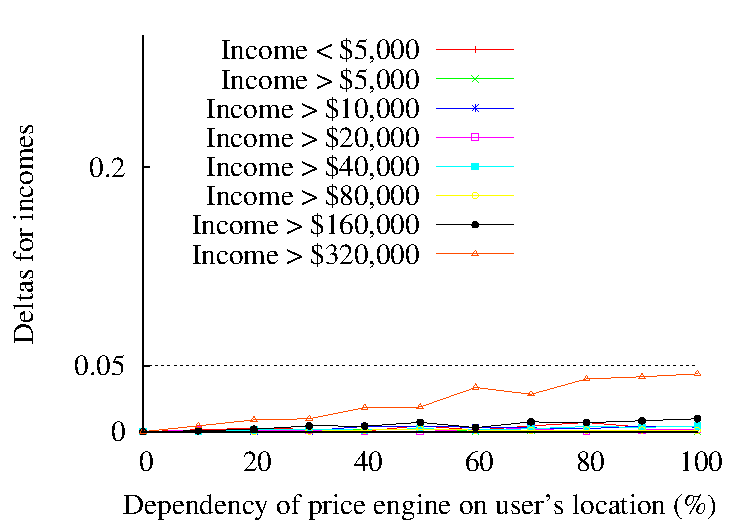
\includegraphics[width=0.33\textwidth]
    {\detokenize{results/income_discrimination_on_location_dependency}}
    \label{fig:}
 }
 \subfigure[Race]{
    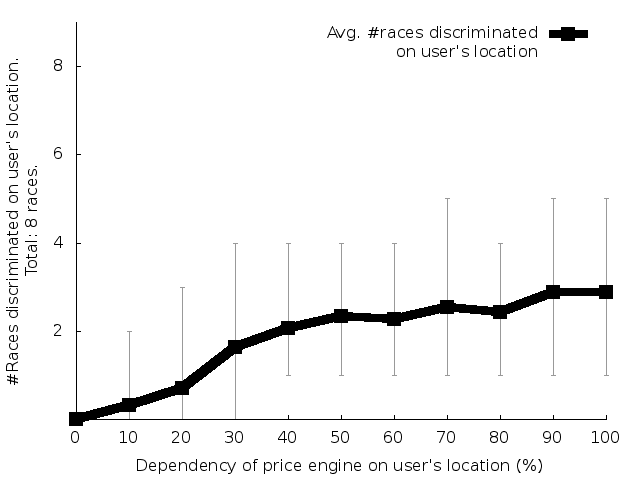
\includegraphics[width=0.33\textwidth]
    {\detokenize{results/race_discrimination_on_location_dependency}}
    \label{fig:}
  }
 \subfigure[Sex]{
    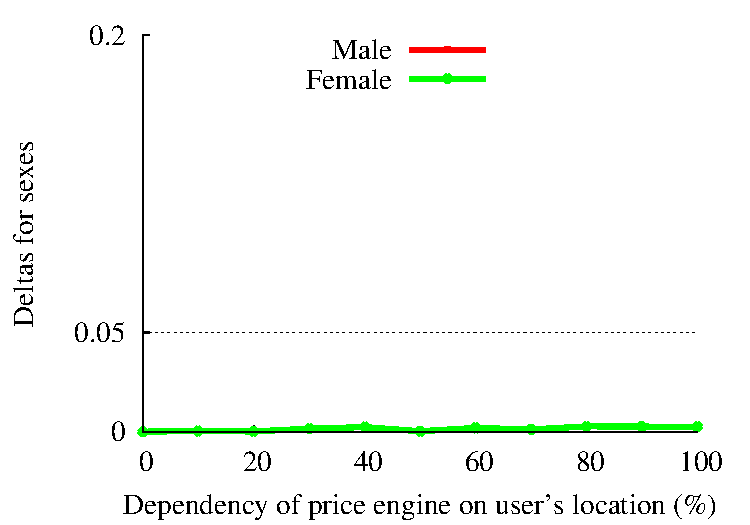
\includegraphics[width=0.33\textwidth]
    {\detokenize{results/sex_discrimination_on_location_dependency}}
    \label{fig:}
  }
 \caption{\textbf{Statistical parity and its dependency on user's location.}
          Shows the dependency of statistical parity, i.e., number of samples that
          violate condition~\ref{eq:StatisticalParity}, as a function of (a) user's income,
          (b) user's race, and (c) user's sex. Figure (b) reveals that statistical parity on
          user-incomes correlates with the dependency of the price engine on user's location.
          While Figures (a) and (b) reveal that statistical parity on user-race and on user-sex
          do not correlate with the dependency of the price engine on user's location.}
}
\end{figure*}


\begin{figure*}[t]
{
 \subfigure[Race]{
    \includegraphics[width=0.33\textwidth]
    {\detokenize{results/race_discrimination_on_proportional}}
    \label{fig:}
  }
  \subfigure[Income]{
    \includegraphics[width=0.33\textwidth]
    {\detokenize{results/income_discrimination_on_proportional}}
    \label{fig:IncomeDiscriminationProportional}
 }
 \subfigure[Sex]{
    \includegraphics[width=0.33\textwidth]
    {\detokenize{results/sex_discrimination_on_proportional}}
    \label{fig:}
  }
 \caption{\textbf{Prices shown to users and their dependency on income, race, and sex.}
          Shows the proportion of high versus low prices shown to users based on income,
          race, and sex. Figure (b) reveals that a users with annual income less than
          \$5,000 receive proportionaly more high prices than users with annual income
          more than \$320,000. Figure (a) indicates that Indian or Alaskan users receive
          notably more high prices than any other race. This raises a consern, since as
          shown in Figure~\ref{fig:IncomePerRace}, an Indian or Alaskan user has a
          considerably lower income than a white American user. Figure (c) shows that
          male and female users receive approximately the same proportion of high versus
          low prices.}
}
\end{figure*}


\begin{figure}[!h]
 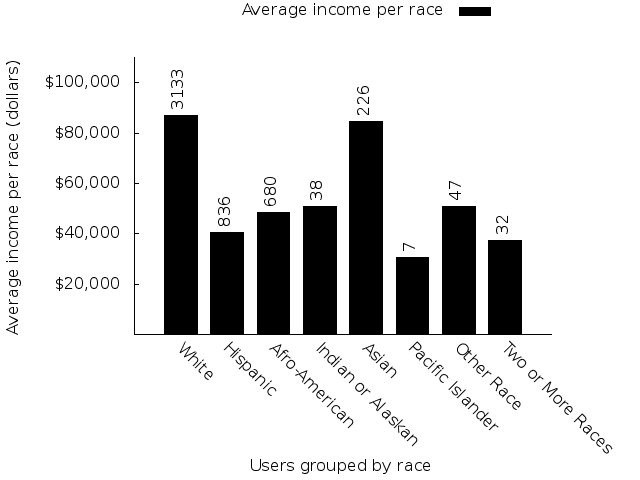
\includegraphics[width=0.49\textwidth]
  {\detokenize{results/income_per_race}}
  \caption{\textbf{Average user income for each race.} An Indian or Alaskan user has
           a considerably lower income than a white American user, and yet, as shown in
           Figure~\ref{fig:IncomeDiscriminationProportional}, he or she receives
           proportional more high prices compared to a white American.}
  \label{fig:IncomePerRace}
\end{figure}

\begin{figure*}[t]
{
 \subfigure[Race]{
    \includegraphics[width=0.33\textwidth]
    {\detokenize{results/misc/race_discrimination_on_proportional}}
    \label{fig:}
  }
  \subfigure[Income]{
    \includegraphics[width=0.33\textwidth]
    {\detokenize{results/misc/income_discrimination_on_proportional}}
    \label{fig:IncomeDiscriminationProportional}
 }
 \subfigure[Sex]{
    \includegraphics[width=0.33\textwidth]
    {\detokenize{results/misc/sex_discrimination_on_proportional}}
    \label{fig:}
  }
 \caption{\textbf{NEW:Prices shown to users and their dependency on income, race, and sex.}
          Shows the proportion of high versus low prices shown to users based on income,
          race, and sex. Figure (b) reveals that a users with annual income less than
          \$5,000 receive proportionaly more high prices than users with annual income
          more than \$320,000. Figure (a) indicates that Indian or Alaskan users receive
          notably more high prices than any other race. This raises a consern, since as
          shown in Figure~\ref{fig:IncomePerRace}, an Indian or Alaskan user has a
          considerably lower income than a white American user. Figure (c) shows that
          male and female users receive approximately the same proportion of high versus
          low prices.}
}
\end{figure*}



